\documentclass[12pt]{article}

\usepackage{amsmath}
\usepackage{hyperref}
\usepackage{graphicx}
\usepackage{float}
\usepackage{caption}
\usepackage{listings}
\usepackage{xcolor}

% Define colors
\colorlet{punct}{red!60!black}
\definecolor{background}{RGB}{240, 248, 255} % Pale Blue
\definecolor{delim}{RGB}{20,105,176}
\colorlet{numb}{magenta!60!black}

% Define JSON language
\lstdefinelanguage{json}{
    basicstyle=\normalfont\ttfamily,
    numbers=left,
    numberstyle=\scriptsize,
    stepnumber=1,
    numbersep=8pt,
    showstringspaces=false,
    breaklines=true,
    frame=lines,
    backgroundcolor=\color{background},
    literate=
     *{0}{{{\color{numb}0}}}{1}
      {1}{{{\color{numb}1}}}{1}
      {2}{{{\color{numb}2}}}{1}
      {3}{{{\color{numb}3}}}{1}
      {4}{{{\color{numb}4}}}{1}
      {5}{{{\color{numb}5}}}{1}
      {6}{{{\color{numb}6}}}{1}
      {7}{{{\color{numb}7}}}{1}
      {8}{{{\color{numb}8}}}{1}
      {9}{{{\color{numb}9}}}{1}
      {:}{{{\color{punct}{:}}}}{1}
      {,}{{{\color{punct}{,}}}}{1}
      {\{}{{{\color{delim}{\{}}}}{1}
      {\}}{{{\color{delim}{\}}}}}{1}
      {[}{{{\color{delim}{[}}}}{1}
      {]}{{{\color{delim}{]}}}}{1},
}



\setlength{\parskip}{1em}

\lstset{frame=single, showstringspaces=false, columns=fixed, basicstyle={\ttfamily}, commentstyle={\it}, numbers=left, tabsize=4}

\definecolor{codebackground}{RGB}{240, 248, 255} % Pale Blue
\definecolor{codecomment}{RGB}{106,153,85}
\definecolor{codekeyword}{RGB}{30,30,255}
\definecolor{codestring}{RGB}{163,21,21}
\definecolor{codenumber}{RGB}{100,100,100}

\lstdefinestyle{modernstyle}{
    backgroundcolor=\color{codebackground},
    commentstyle=\color{codecomment},
    keywordstyle=\color{codekeyword},
    numberstyle=\tiny\color{codenumber},
    stringstyle=\color{codestring},
    basicstyle=\ttfamily\footnotesize\color{black},
    breakatwhitespace=false,
    breaklines=true,
    captionpos=b,
    keepspaces=true,
    numbers=left,
    numbersep=5pt,
    showspaces=false,
    showstringspaces=false,
    showtabs=false,
    tabsize=4
}

\lstset{style=modernstyle}

\begin{document}

\begin{titlepage}
\centering
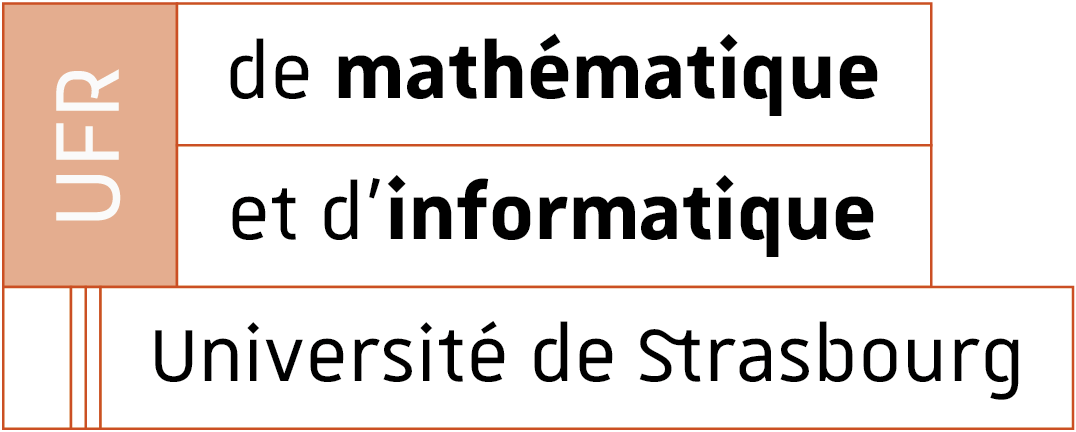
\includegraphics[width=0.5\textwidth]{images/logo_ufr.png}\par\vspace{1cm}
\vspace{1.5cm}
{\huge\bfseries ExaMA WP1 - Vegetation\par}
\vspace{2cm}
{\Large Giulio Carpi Lapi, Pierre-Antoine Senger\par}
\vfill
supervised by\par
Pierre Alliez and Vincent Chabannes

\vfill

% Bottom of the page
{\large Date: \today\par}
\end{titlepage}

\tableofcontents
\newpage

\section{Introduction}
Urban areas are complex ecosystems influenced by various factors, among which
vegetation, especially trees, holds significant importance. Trees play a crucial
role in shaping microclimates, reducing energy consumption, and enhancing overall
livability\cite{TIR4sTREEt}. This project aims to integrate vegetation, specifically trees, into 3D
geometric models of urban environments to improve the accuracy and realism of thermal
and energy simulations. Utilizing data from open sources like \texttt{OpenStreetMap},
we identified tree positions and attributes and developed a library of 3D tree
models for integration into terrain meshes.

The project follows a roadmap with defined milestones to deliver versions
\texttt{V0}, \texttt{V1}, and \texttt{V2} by specified  deadlines.

\subsection{Main objectives}

The primary objective is to enhance the accuracy of thermal and energy
simulations of a given area.

Specific objectives include:
\begin{itemize}
    \item Extracting tree data from \texttt{OpenStreetMap}
    \item Generating 3D tree models.
    \item Integrating tree models into terrain meshes.
    \item Simulating how trees influence energy consumption and microclimates.
    \item Optimizing computational efficiency
    \item Delivering versions \texttt{V0}, \texttt{V1}, and \texttt{V2} by specified deadlines
\end{itemize}

\begin{figure}[H]
    \centering
    \begin{minipage}{0.45\textwidth}
        \centering
        \includegraphics[width=\textwidth]{images/TreeShade.png}
        \captionsetup{font={scriptsize}}
        \caption{Tree providing shade to a building \cite{img:TreeShade}.}
    \end{minipage}\hfill
    \begin{minipage}{0.45\textwidth}
        \centering
        \includegraphics[width=\textwidth]{images/heat_street.png}
        \captionsetup{font={scriptsize}}
        \caption{Thermal image of a street depicting heat distribution \cite{img:street_thermography}.}
    \end{minipage}
\end{figure}

Computational modeling has advanced significantly, enabling the simulation of thermal
and energy performance in urban environments. However, integrating vegetation into
these models presents challenges due to the complexity of obtaining accurate tree data
and representing their geometry efficiently\cite{AdTree}.

\newpage

\subsection{Challenges}
This project aims to address these challenges by developing a methodology for
integrating trees into 3D urban models. Leveraging data from \texttt{OpenStreetMap},
the  project will identify tree positions and attributes, generate a library of 3D tree
models, and integrate them into terrain meshes for comprehensive simulations while
ensuring computational efficiency.

One of the main challenges is to developp a way to represent different density
of leaves for each season. To streamline things, we've opted to combine spring
and summer into one period and fall and winter into another, giving us just two
seasons. The first boasts dense foliage, while the second experiences sparse leaf coverage.
This could be done by adding multiple textures to the tree mesh and changing
the texture based on the season.

\subsection{Data formats and structure}
Tree data will be sourced from \texttt{OpenStreetMap} and processed into formats suitable for
integration into our models, such as \texttt{.stl}, \texttt{.csv}, and \texttt{.json}.
We aim to ensure watertight triangulation consistent with the Finite Element Method
(FEM) for accurate simulations.

The \texttt{stl} format\cite{stl_format} is a widely used format for 3D printing and computer-aided design (CAD)
software. It represents 3D models as a collection of triangular facets, making it
suitable for our geometric modeling purposes.
The \texttt{ASCII} versions is defined as :
\begin{lstlisting}
solid name
facet normal ni nj nk
    outer loop
        vertex v1x v1y v1z
        vertex v2x v2y v2z
        vertex v3x v3y v3z
    endloop
endfacet
....
endsolid name
\end{lstlisting}
But for efficiency we will use the \texttt{stl} format in its \textbf{binary form}.
\subsection{Software and libraries}
To source our data, we'll utilize the \texttt{Overpass API} \cite{overpass} alongside
\texttt{curl} \cite{curl} to access and leverage information from \texttt{OpenStreetMap}.
For geometric modeling, we will utilize the \texttt{CGAL} library, known for its efficiency and
reliability in geometric computation\cite{cgal}. Shading calculations will be performed using the
\texttt{Feel++} \cite{feel++} library, which specializes in solving Partial Differential Equations (PDEs)
essential for simulating light and shade on 3D objects.

\subsection{GitHub repository}
We created a \href{https://github.com/master-csmi/2024-m1-vegetation}{GitHub} repository to manage the project and facilitate collaboration.
The repository contains the project's code, documentation, and resources. It will be
updated regularly to reflect the progress and changes made during the project's
development.

\subsection{Roadmap}
The roadmap we defined includes the following milestones and issues:

\begin{figure}[H]
    \centering
    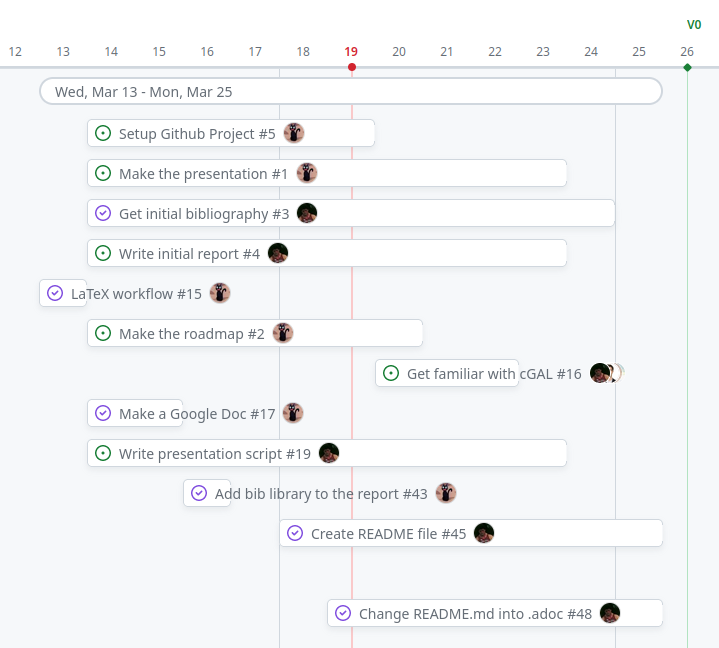
\includegraphics[width=1\textwidth]{images/roadmap_v0.png}
    \captionsetup{font={scriptsize}}
    \caption{Roadmap for V0}
\end{figure}

\begin{figure}[H]
    \centering
    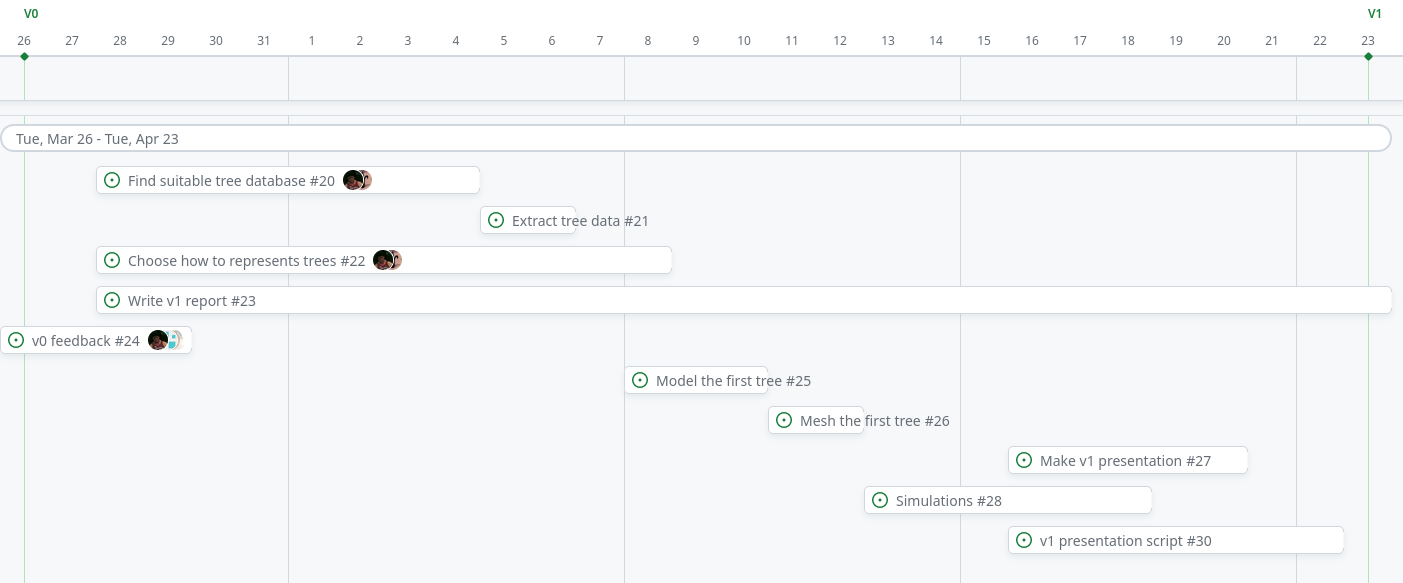
\includegraphics[width=1\textwidth]{images/roadmap_v1.png}
    \captionsetup{font={scriptsize}}
    \caption{Roadmap for V1}
\end{figure}

\begin{figure}[H]
    \centering
    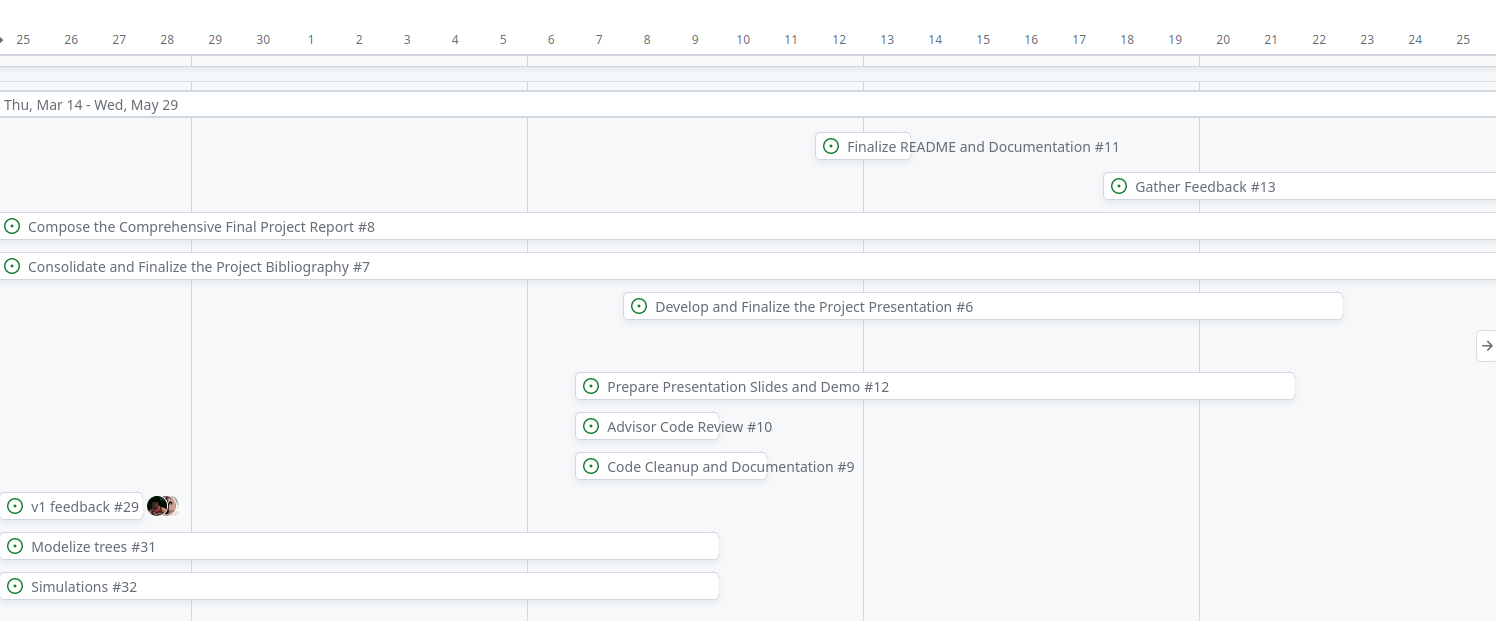
\includegraphics[width=1\textwidth]{images/roadmap_v2.png}
    \captionsetup{font={scriptsize}}
    \caption{Roadmap for V2}
\end{figure}

\newpage

\section{Methodology}

\subsection{Data acquisition}
A \textit{config.json} file will be available for the user to specify the area of
interest and some parameters for the tree generation. \\

\begin{lstlisting}[language=json]
{
    "bbox": "48.5866,7.7522,48.5876,7.7557",
    "origin": "48.583055227464364, 7.748664426560083",
    "LOD": 0,
    "default_height": 10,
    "default_genus": "Platanus",
    "input_building_mesh": "mesh_lod1.stl",
    "output_name": "republique"
}
\end{lstlisting}

Where :
\begin{itemize}
    \item \texttt{bbox} is the bounding box for the query in the format:
    \subitem (bottom latitude, bottom longitude, top latitude, top longitude)
    \item \texttt{origin} is the origin of the 3D space in latitude and longitude
    used to convert the GPS coordinates to Cartesian coordinates.
    \item \texttt{LOD} is the level of details of the meshes (0, 1, 2 or 3)
    \item \texttt{default\_height} is the default height of the trees if not specified in the data.
    \item \texttt{default\_genus} is the default genus of the trees if not specified in the data.
    \item \texttt{input\_building\_mesh} is the name of the input file representing the building mesh.
    \item \texttt{output\_name} is the name of the output file representing the unions of the tree meshes.
\end{itemize}


We will then use the \texttt{Overpass API} to query \texttt{OpenStreetMap}
for all the available tree data within the specified bounding box.
The data will be stored in a \textit{.json} file.

\newpage
Here's an example of the result of the query for one tree:

\begin{lstlisting}[language=json]
{
    "type": "node",
    "id": 10161978695,
    "lat": 48.5872478,
    "lon": 7.7548520,
    "tags": {
        "circumference": "78.54",
        "diameter_crown": "5",
        "genus": "Tilia",
        "height": "10",
        "natural": "tree",
        "ref": "27466",
        "source": "data.strasbourg.eu - patrimoine_arbore",
        "source:date": "2022-01-02",
        "species": "Tilia euchlora x"
    }
}
\end{lstlisting}

We will especially use the \texttt{position} of the tree (latitude and longitude),
its \texttt{height} and the \texttt{genus} (since this data is more abundant than the species)
to generate the 3D tree models.

\subsection{Tree library}
Using the results from the \texttt{Overpass API} query, we will create a library
of tree objects. Each tree object will contain the tree's metadata (location, species, height,
leave density, etc.).

Additionally, since it's not feasible to have a mesh model for each species of trees, 
we will use the \texttt{trees.json} file to specify the genus categories for the
 meshing of the trees. \\

\newpage

\begin{lstlisting}[language=json]
{
    "known_genus": [
        "Abies",
        "Acer",
        "Aesculus",
        ...
    ],
    "cedrus_like": [
        "Chaemacyparis",
        "Cupressus",
        ...
    ],
    "acer_like": ["Fadus", "Metasequoia", "Sequoiadendron", "Thuja", "Tsuga"],
    "liquidambar_like": ["Liriodendron", "Pyrus", "Alnus", "Ostrya"],
    "quercus_like": [
        "Corylus",
        "Carya",
        "Fagus",
        ...
    ]
}
\end{lstlisting}

\begin{itemize}
    \item \texttt{known\_genus} is a list of the genus for which we have a mesh model.
    \item \texttt{cedrus\_like} is a list of the genus for which the cedrus mesh model will be used.
    \item etc.
\end{itemize}

\subsection{Base tree model}
Since making all tree model would take too much time we will use tree meshes 
publicly available on \href{https://app.sketchup.com/app}{Sketchup} 3D Warehouse.

\begin{figure}[H]
    \centering
        \centering
        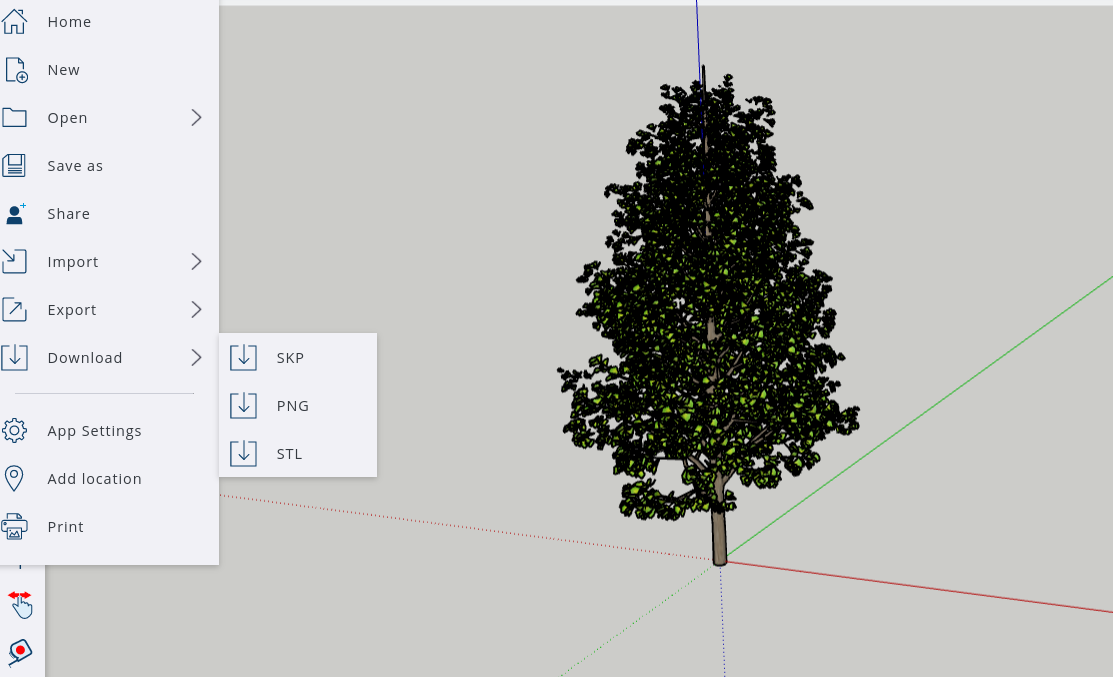
\includegraphics[width=\textwidth]{images/ginkgo_sketchup.png}
        \captionsetup{font={scriptsize}}
        \caption{The mesh of a Ginkgo tree available on Sketchup 3D Warehouse}
\end{figure}

Those meshes can be directly downloaded in STL format\cite{stl_format}.  \\
Below, some of these models visualized using MeshLab\cite{meshlab}:

\begin{figure}[H]
    \centering
    \begin{minipage}{0.24\textwidth}
        \centering
        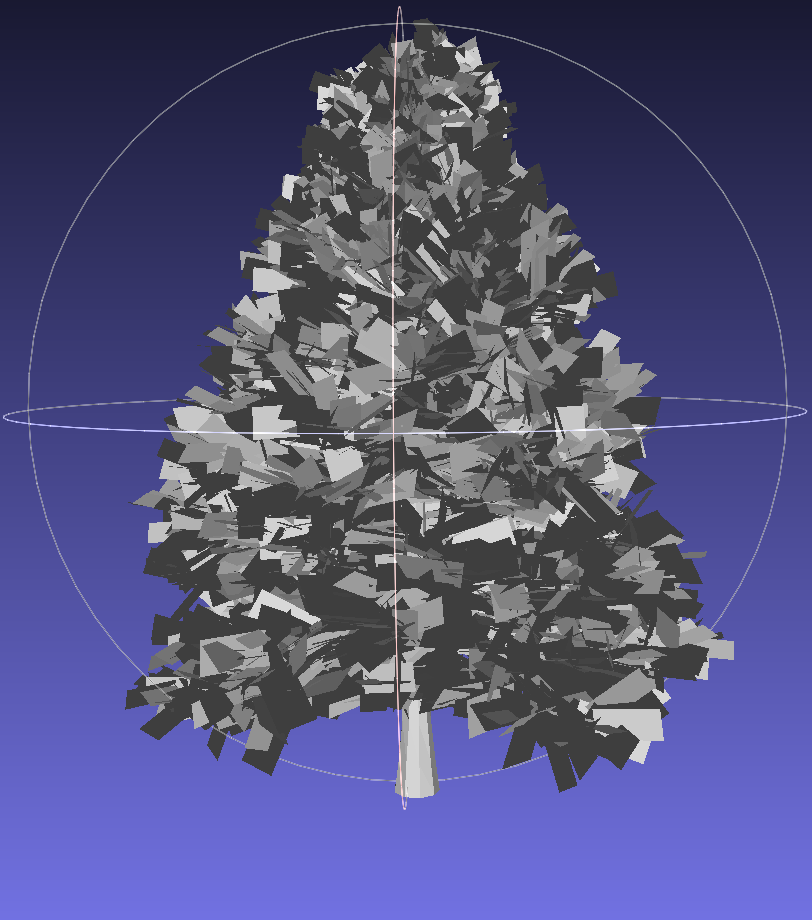
\includegraphics[width=\textwidth]{images/abies.png}
        \captionsetup{font={scriptsize}}
        \caption{Abies.}
    \end{minipage}\hfill
    \begin{minipage}{0.24\textwidth}
        \centering
        \includegraphics[width=\textwidth]{images/acer.png}
        \captionsetup{font={scriptsize}}
        \caption{Acer.}
    \end{minipage}\hfill
    \begin{minipage}{0.24\textwidth}
        \centering
        \includegraphics[width=\textwidth]{images/aesculus.png}
        \captionsetup{font={scriptsize}}
        \caption{Aesculus.}
    \end{minipage}\hfill
    \begin{minipage}{0.24\textwidth}
        \centering
        \includegraphics[width=\textwidth]{images/catalpa.png}
        \captionsetup{font={scriptsize}}
        \caption{Catalpa.}
    \end{minipage}
\end{figure}

\begin{figure}[H]
    \centering
    \begin{minipage}{0.24\textwidth}
        \centering
        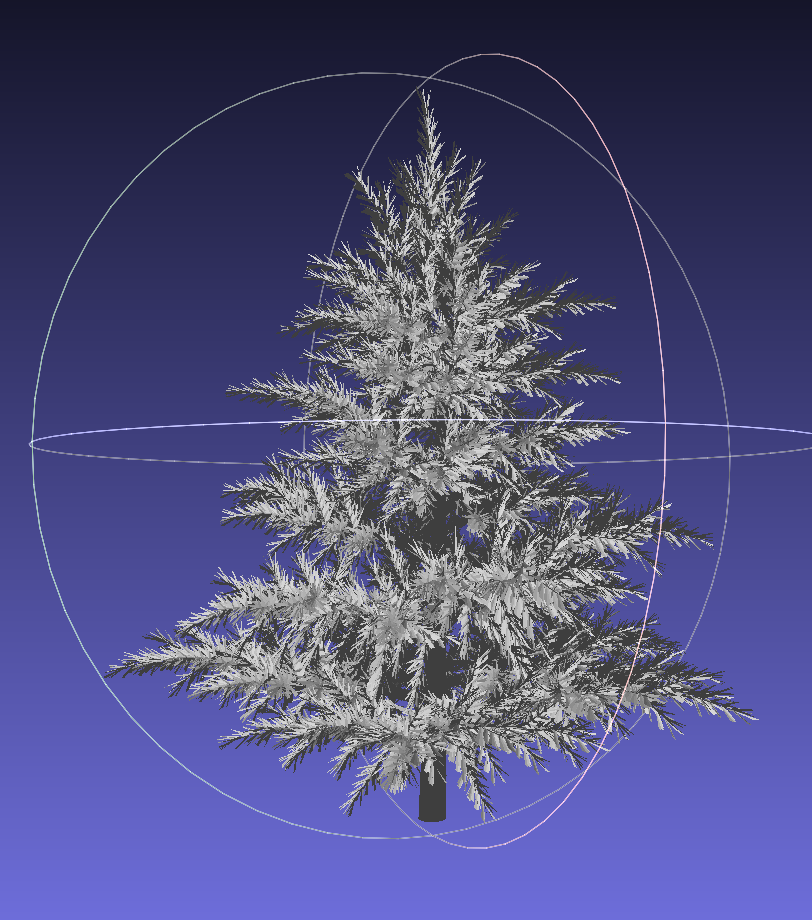
\includegraphics[width=\textwidth]{images/cedrus.png}
        \captionsetup{font={scriptsize}}
        \caption{Cedrus.}
    \end{minipage}\hfill
    \begin{minipage}{0.24\textwidth}
        \centering
        \includegraphics[width=\textwidth]{images/liquidanbar.png}
        \captionsetup{font={scriptsize}}
        \caption{Liquidanbar.}
    \end{minipage}\hfill
    \begin{minipage}{0.24\textwidth}
        \centering
        \includegraphics[width=\textwidth]{images/platanus.png}
        \captionsetup{font={scriptsize}}
        \caption{Platanus.}
    \end{minipage}\hfill
    \begin{minipage}{0.24\textwidth}
        \centering
        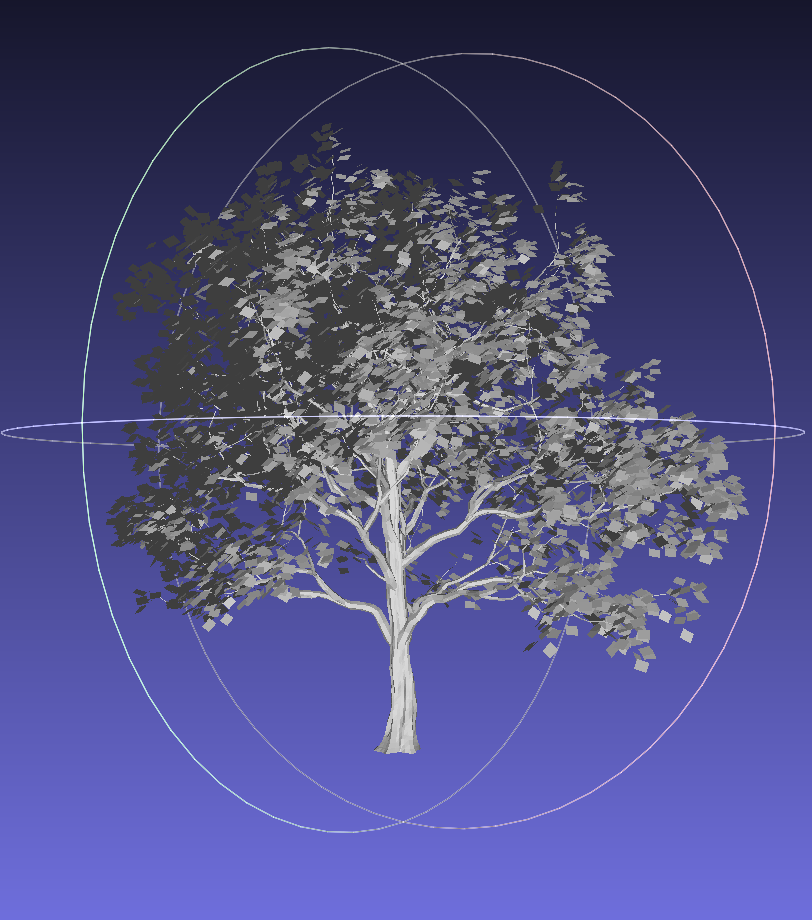
\includegraphics[width=\textwidth]{images/quercus.png}
        \captionsetup{font={scriptsize}}
        \caption{Quercus.}
    \end{minipage}
\end{figure}

To provide different level of details (LOD) we will wrap them using the
CGAL 3D Alpha Wrapping\cite{cgal_alpha_wrapper}.

\subsection{Alpha Wrapping}
\begin{figure}[H]
    \centering
        \centering
        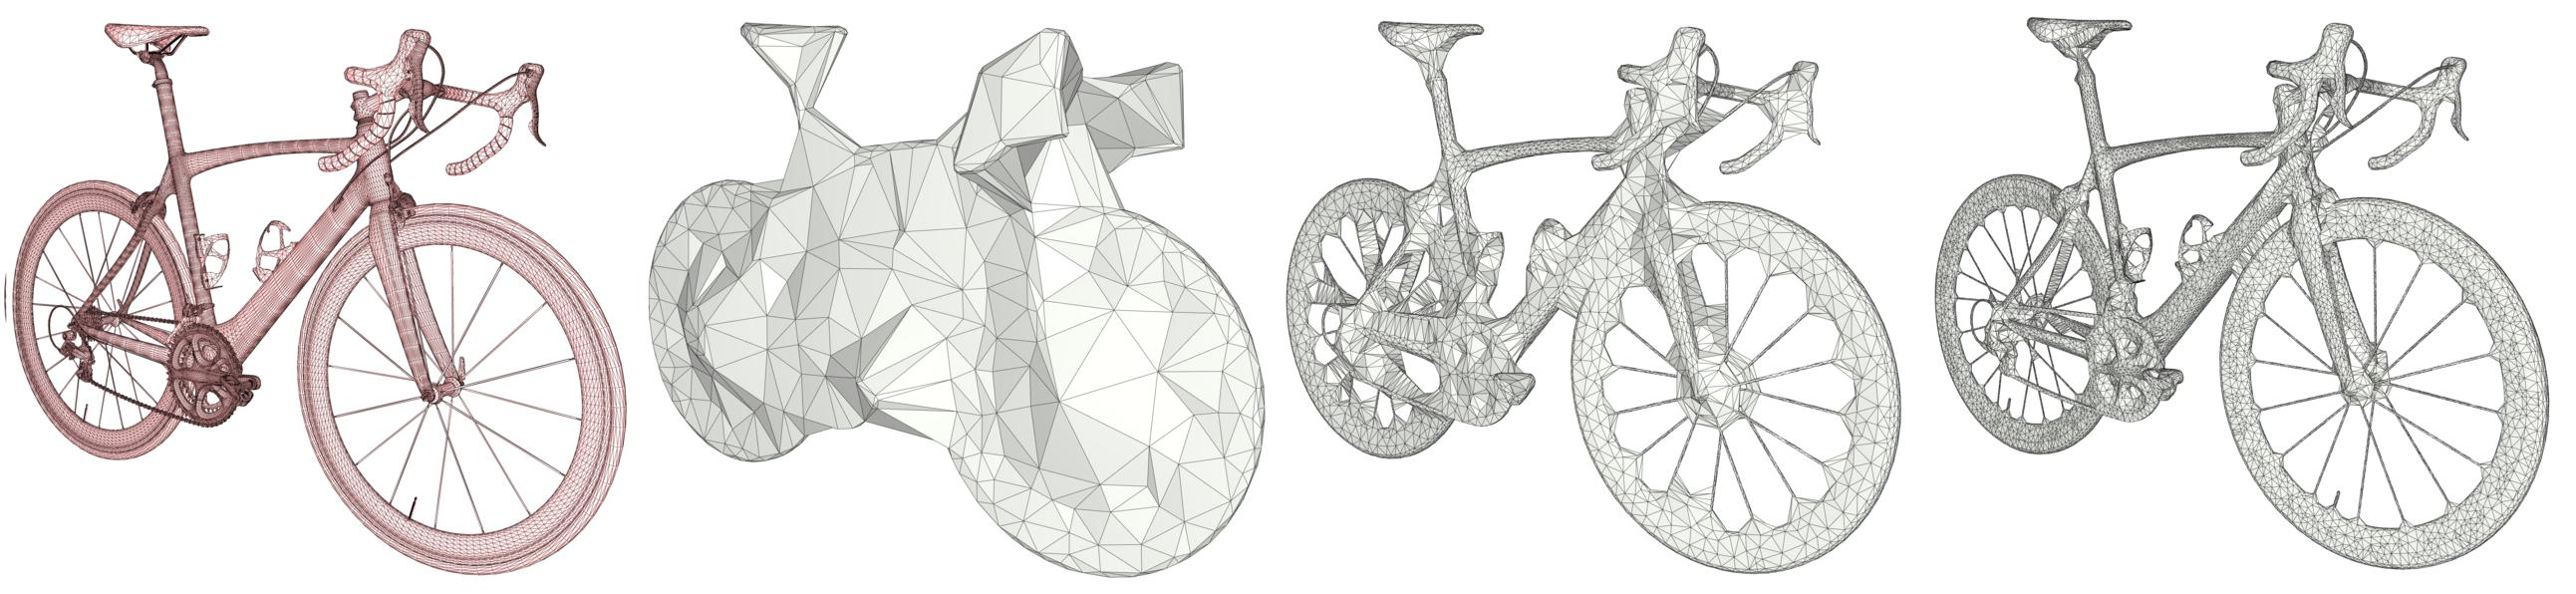
\includegraphics[width=\textwidth]{images/aw3_bike_lod.jpg}
        \captionsetup{font={scriptsize}}
        \caption{Different LOD of the Alpha Wrapping of a bike}
\end{figure}

\textbf{Approach}\\
Many approaches exist to enclose a 3D model within a volume, each balancing runtime
and quality (tightness) of approximation. Simple methods, like using an axis-aligned
or oriented bounding box, have uncontrollable and often large approximation errors.
Computing the convex hull of the input improves quality but increases runtime and
still provides a crude approximation, especially for models with several components.

The convex hull is a special case of alpha shapes. Mathematically, alpha shapes are
subcomplexes of the Delaunay triangulation, where simplices are included based on the
size of their minimal (empty) Delaunay ball. Constructing 3D alpha shapes can be seen
as carving 3D space with an empty ball of radius alpha. Alpha shapes provide good
piecewise-linear approximations of a shape but are defined on point sets. For more
general input data like triangle soups, even after sampling, alpha shapes may not be
conservative for any alpha and can carve inner structures within volumes.

Inspired by alpha shapes, we use shrink-wrapping. We iteratively construct a subcomplex
of a 3D Delaunay triangulation by starting from a simple triangulation enclosing the
input and then iteratively removing eligible tetrahedra on the boundary of the complex.
The underlying triangulation is refined as shrinking proceeds. Instead of carving from
the convex hull, we construct a new mesh through a Delaunay refinement-like algorithm.
This algorithm inserts Steiner points on the boundary of an offset volume, defined as
a level set of the unsigned distance field to the input.

This method prevents the creation of inner structures and avoids superfluous
computations. It also detaches mesh construction from the input's geometry and
discretization, offering several advantages: (1) the input format is flexible (triangle
soups, polygon soups, point clouds), as only three basic geometric queries are needed:
(a) the distance between a point and the input, (b) the projection of a query point
onto the input, and (c) an intersection test between a tetrahedron and the input, and
(2) the user can trade tightness to the input for final mesh complexity, requiring
fewer mesh elements for a large offset conservative approximation.

\textbf{Algorithm Initialization}\\
The algorithm begins by inserting the eight corner vertices of a loose bounding box
into a 3D Delaunay triangulation. In CGAL's 3D Delaunay triangulation, all triangle
facets are adjacent to two tetrahedron cells. Each boundary facet of the triangulation,
coinciding with a convex hull facet, is adjacent to an infinite tetrahedron cell.
Initially, all infinite cells are tagged as outside, and all finite tetrahedron cells
are tagged as inside.

\textbf{Shrink-wrapping}\\
The algorithm traverses the cells of the Delaunay triangulation from outside to inside,
flood-filling from one cell to its adjacent cell and tagging the adjacent cell as
outside when possible. Flood-filling uses a priority queue of Delaunay triangle facets
(gates) representing the traversal between adjacent cells.

A gate is alpha-traversable if its circumradius is larger than the user-defined
parameter alpha, where the circumradius is the radius of the relating triangle's
Delaunay ball. Cavities smaller than alpha are not accessible as their gates are not
alpha-traversable.

Initialized by the alpha-traversable gates on the convex hull, the priority queue only
contains alpha-traversable gates and is sorted by decreasing circumradius. Traversal
advances along dual Voronoi edges of the gates with a pencil of empty balls
circumscribing the gate.

\begin{figure}[H]
    \centering
        \centering
        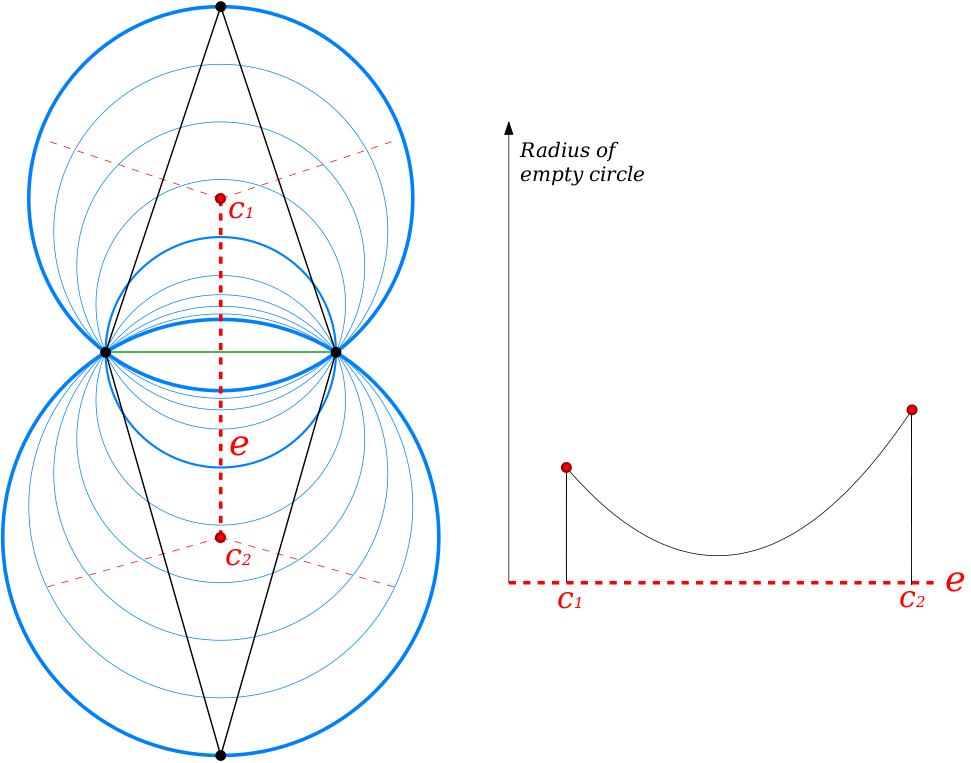
\includegraphics[width=\textwidth]{images/aw3_pencil.png}
        \captionsetup{font={scriptsize}}
        \caption{(Left) Pencil of empty circles (blue) circumscribing a Delaunay 
        edge (green) in a 2D Delaunay triangulation (black). From the top triangle 
        circumcenter c1 to the bottom triangle circumcenter c2, the dual Voronoi
         edge denoted by e (doted red) is the trace of centers of the largest circles
          that are empty of Delaunay vertex. (Right) The graph corresponding to the 
          left example. The x-axis corresponds to the position of empty circle centers
           located on the Voronoi edge e, from c1 to c2. The y-axis is the radius
            value of the corresponding empty circles. In this case, the minimum 
            radius of this pencil of empty circle is located at the midpoint of 
            the green Delaunay edge. In our algorithm, a gate (green Delaunay edge)
             is said to be not alpha-traversable when the minimum radius of the pencil
              of empty circle is smaller than alpha. }
\end{figure}

When traversing from an outside cell \( c_o \) to an inside cell \( c_i \) through an 
alpha-traversable facet \( f \), two criteria are tested to prevent the wrapping process 
from colliding with the input:

1. Check for an intersection between the dual Voronoi edge of \( f \) and the offset 
surface, defined as the level set of the unsigned isosurface to the input. If intersections 
exist, the first intersection point along the dual Voronoi edge oriented from outside to 
inside is inserted into the triangulation as a Steiner point.

2. If the dual Voronoi edge does not intersect the offset surface but the neighboring cell 
\( c_i \) intersects the input, compute the projection of the circumcenter of \( c_i \) 
onto the offset surface and insert it into the triangulation as a Steiner point, which 
destroys \( c_i \).

After each Steiner point insertion, all new incident cells are tagged as inside, and the 
newly alpha-traversable gates are pushed into the priority queue.

If neither criterion is met, the neighboring cell \( c_i \) is traversed and tagged as 
outside. Alpha-traversable facets of \( c_i \) separating inside from outside cells are 
pushed as new gates into the priority queue.

Once the queue empties—a process guaranteed as facets (and their circumradii) become 
smaller due to new Steiner point insertions—the construction phase terminates. The output 
triangle surface mesh is extracted from the Delaunay triangulation as the set of facets 
separating inside from outside cells.

The figure below depicts the steps of the algorithm in 2D.
\begin{figure}[H]
    \centering
        \centering
        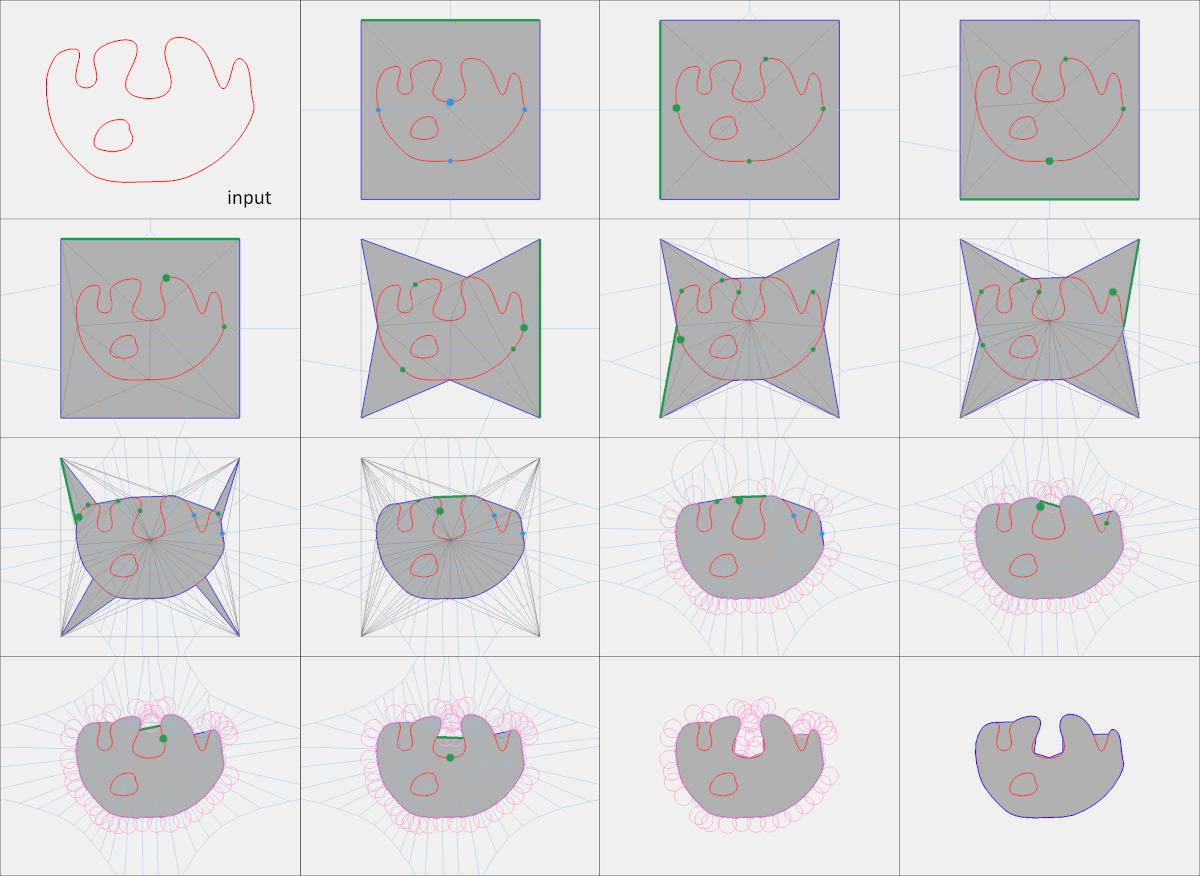
\includegraphics[width=\textwidth]{images/aw3_steps.jpg}
        \captionsetup{font={scriptsize}}
        \caption{Steps of the shrink-wrapping algorithm in 2D. The algorithm is initialized by 
        inserting the corners of the loose bounding box of the input (red) into a Delaunay 
        triangulation, and all finite triangles are tagged inside (grey). The current gate 
        (green edge) popped out from the queue is alpha-traversable. The triangle adjacent 
        to the gate is tagged outside when it does not intersect the input, and new 
        alpha-traversable gates are pushed to the queue. When the adjacent triangle 
        intersects the input, a new Steiner point (large green disc) is computed and inserted 
        into the triangulation, all neighboring triangles are tagged inside, new 
        alpha-traversable gates are pushed to the queue, and traversal is resumed. Grey edges 
        depict the Delaunay triangulation. Blue edges depict the Voronoi diagram. Pink circles 
        depict the empty circle of radius alpha. The output edges (dark blue) separate inside 
        from outside triangles.
        }
\end{figure}

\textbf{Guarantees} \\
The algorithm is proven to terminate and to produce a 2-manifold triangulated surface 
mesh that strictly encloses the input data. The key element to the proof is that we wrap 
from outside to inside and never allow a cell that intersects the input to be flagged 
inside. Furthermore, both criteria that lead to refinement of the triangulation insert
 Steiner points that are guaranteed to break the cells in need of refinement and 
 reduce the neighbor facets circumradii.


\subsection{Tree model generation}
Using the CGAL 3D Alpha Wrapping \cite{cgal_alpha_wrapper} algorithm we will produce
reference tree meshes for each level of detail (LOD) from 0 to 3 to avoid computing
a new mesh for each tree.

A \texttt{wrap} executable will be available to generate the reference meshes, it 
can be used as follows:
(50 is the alpha value and 600 is the offset value)

\begin{lstlisting}[language=bash]
./build/wrap tree_ref/raw_tree/Ginkgo.stl 50 600
\end{lstlisting}


Additionally, to wrap all the trees in a directory, the \texttt{wrap\_all.sh} script
can be used:

\begin{lstlisting}[language=bash]
#!/bin/bash

# Directory containing the raw STL files
INPUT_DIR="tree_ref/raw_tree"

# The alpha value to use for wrapping
ALPHA=100

# Loop through all STL files in the input directory
for input_file in $INPUT_DIR/*.stl; do
	./build/wrap "$input_file" "$ALPHA"
done
\end{lstlisting}

To run the script:
\begin{lstlisting}
./wrap_all.sh
\end{lstlisting}

   Those reference meshes will be used to generate the tree models for each tree 
in the data. The tree models will be generated by scaling the reference mesh 
to match the tree's height and position in the 3D space. \\
This will be done by using the \texttt{CGAL Affine Transformation} \cite{cgal_affine_transformation}
which as a linear complexity in the number of vertices of the mesh.

\begin{figure}[H]
    \centering
    \begin{minipage}{0.45\textwidth}
        \centering
        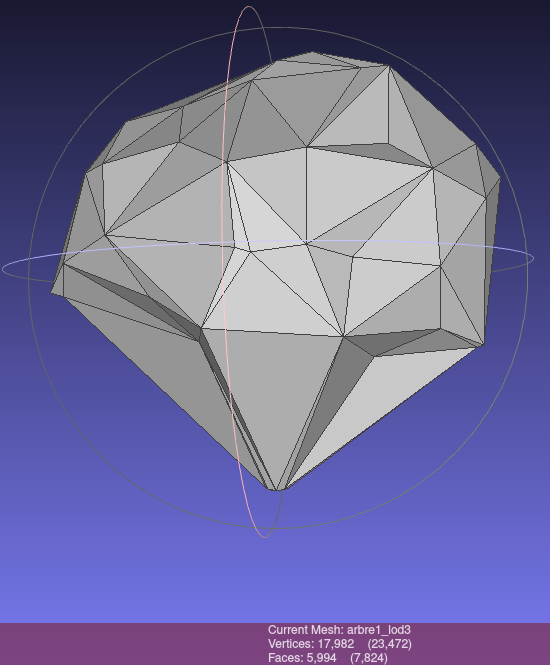
\includegraphics[width=\textwidth]{images/lod0.png}
        \captionsetup{font={scriptsize}}
        \caption{A reference mesh tree for LOD 0.}
    \end{minipage}\hfill
    \begin{minipage}{0.45\textwidth}
        \centering
        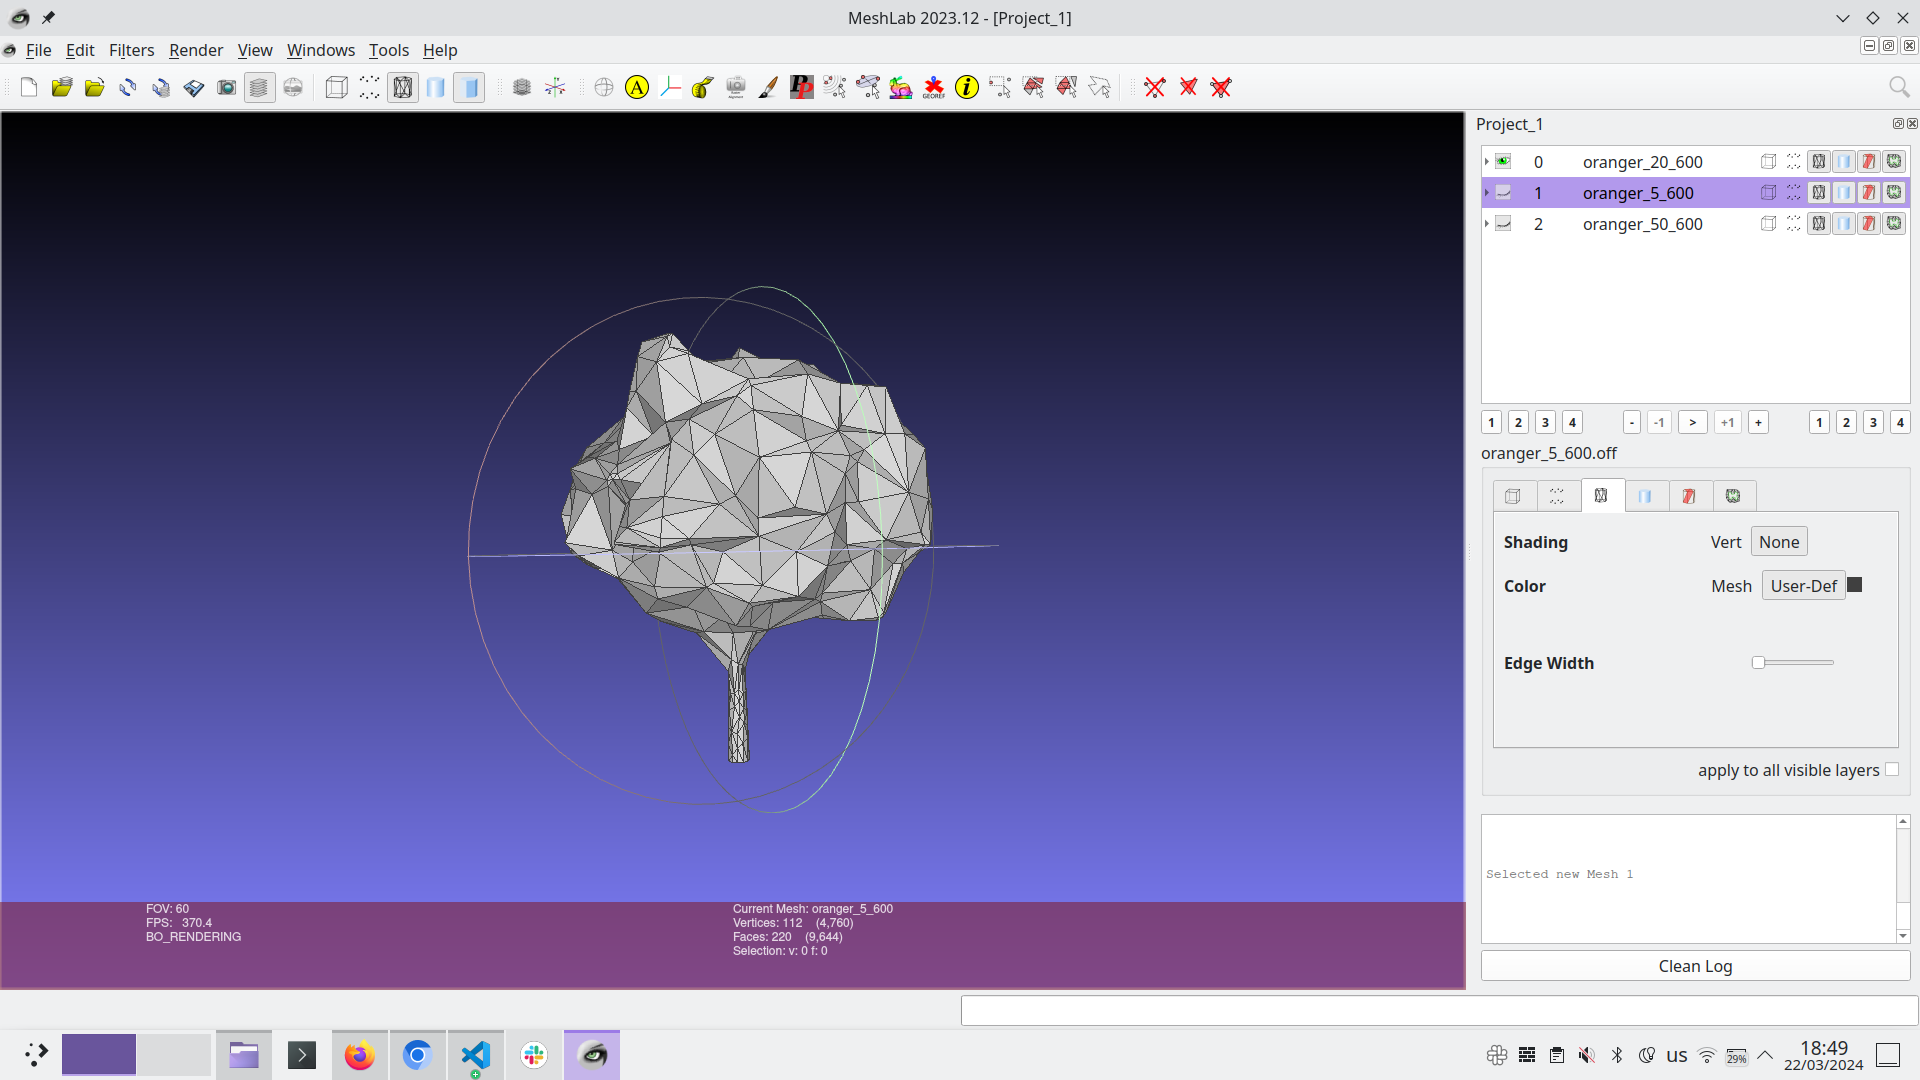
\includegraphics[width=\textwidth]{images/lod1.png}
        \captionsetup{font={scriptsize}}
        \caption{A reference mesh tree for LOD 1.}
    \end{minipage}
\end{figure}

\begin{figure}[H]
    \centering
    \begin{minipage}{0.45\textwidth}
        \centering
        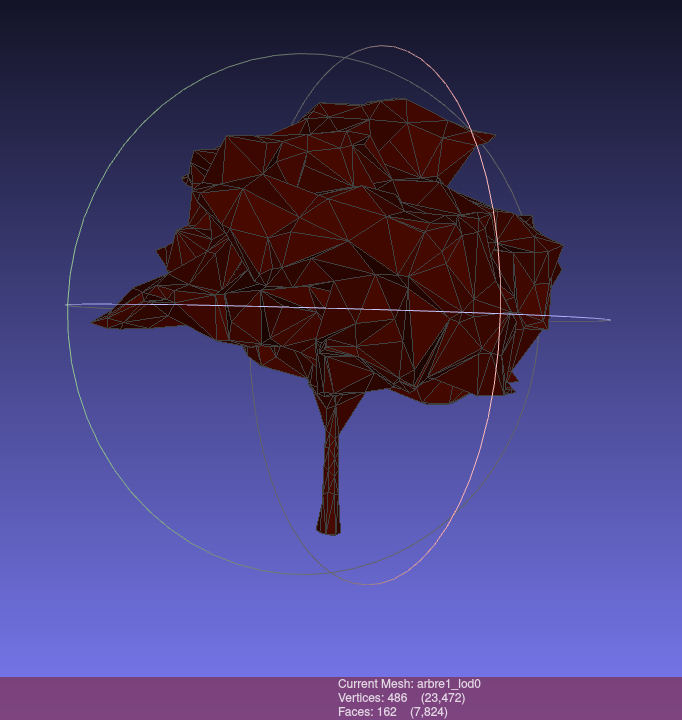
\includegraphics[width=\textwidth]{images/lod2.png}
        \captionsetup{font={scriptsize}}
        \caption{A reference mesh tree for LOD 2.}
    \end{minipage}\hfill
    \begin{minipage}{0.45\textwidth}
        \centering
        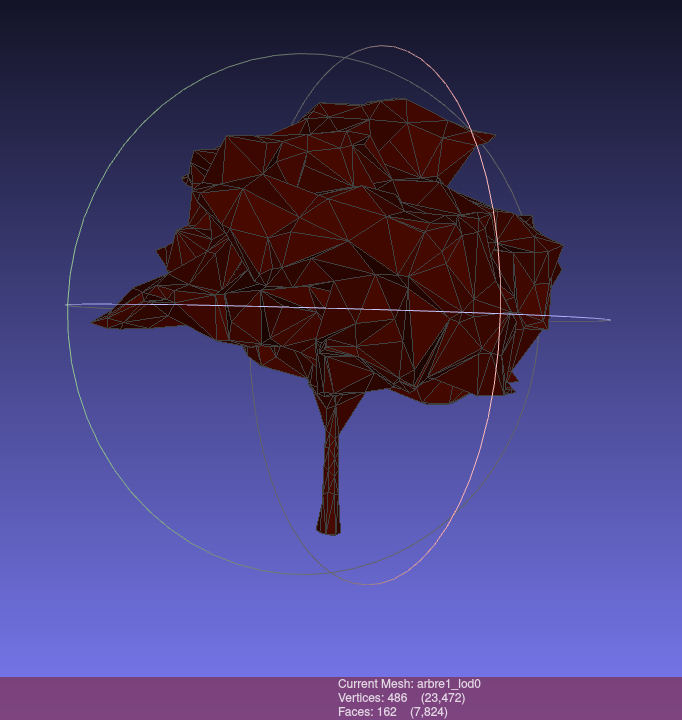
\includegraphics[width=\textwidth]{images/lod3.png}
        \captionsetup{font={scriptsize}}
        \caption{A reference mesh tree for LOD 3.}
    \end{minipage}
\end{figure}

The case where not enough data is available for a tree will need to be handled
as well. \\
Our first idea was to use a k-nearest neighbors algorithm \cite{k-NN} approach to
decide the tree's metadata (species, height, leave density, etc.) based on the
surrounding trees. \\
Unfortunately, this approach is not feasible due to the fact that
when data is missing it's usually missing for a large area such as a park. \\
Instead, we will use first try to use the mean of the available height per genus. \\
Else we will use the default height and genus specified in the \textit{config.json} file.

\subsection{Model integration}
Generated tree models will be integrated into terrain meshes to create comprehensive
3D urban models. To ensure precise integration into the terrain mesh (especially for large area), the tree models coordinates
(latitude, longitude) will be converted to Cartesian coordinates (x, y) using
a Mercator projection\cite{mercator-proj}. To achieve this we will assume the Earth is a geodesic
defined as WGS84 \cite{wgs84} and use the WGS84toCartesian\cite{wgs84_to_cartesian} open source header-only
  library to convert the coordinates.

The union of all the tree meshed need to be computed to create a single mesh
and avoid collision between the trees. \\
This will be achieved using the \href{https://doc.cgal.org/latest/Polygon_mesh_processing/group__PMP__corefinement__grp.html}{corefine\_and\_compute\_union} function from the CGAL library.
(complexity ?) \\
Another approach could be to use the convex hull of the tree meshes, using the 
intersection of the convex hulls to compute the union of the tree meshes.

Here is an example of the tree mesh union of Place de la République in Strasbourg
using generic trees and LOD1:

\begin{figure}[H]
    \centering
        \centering
        \includegraphics[width=\textwidth]{images/mesh_vs_overpass.png}
        \captionsetup{font={scriptsize}}
        \caption{Top view of Place de la République, on the left the mesh generated from the data,
        on the right the overpass data.}

\end{figure}


We were given a \texttt{.stl} file representing the city center of Strasbourg, France.

\begin{figure}[H]
    \centering
    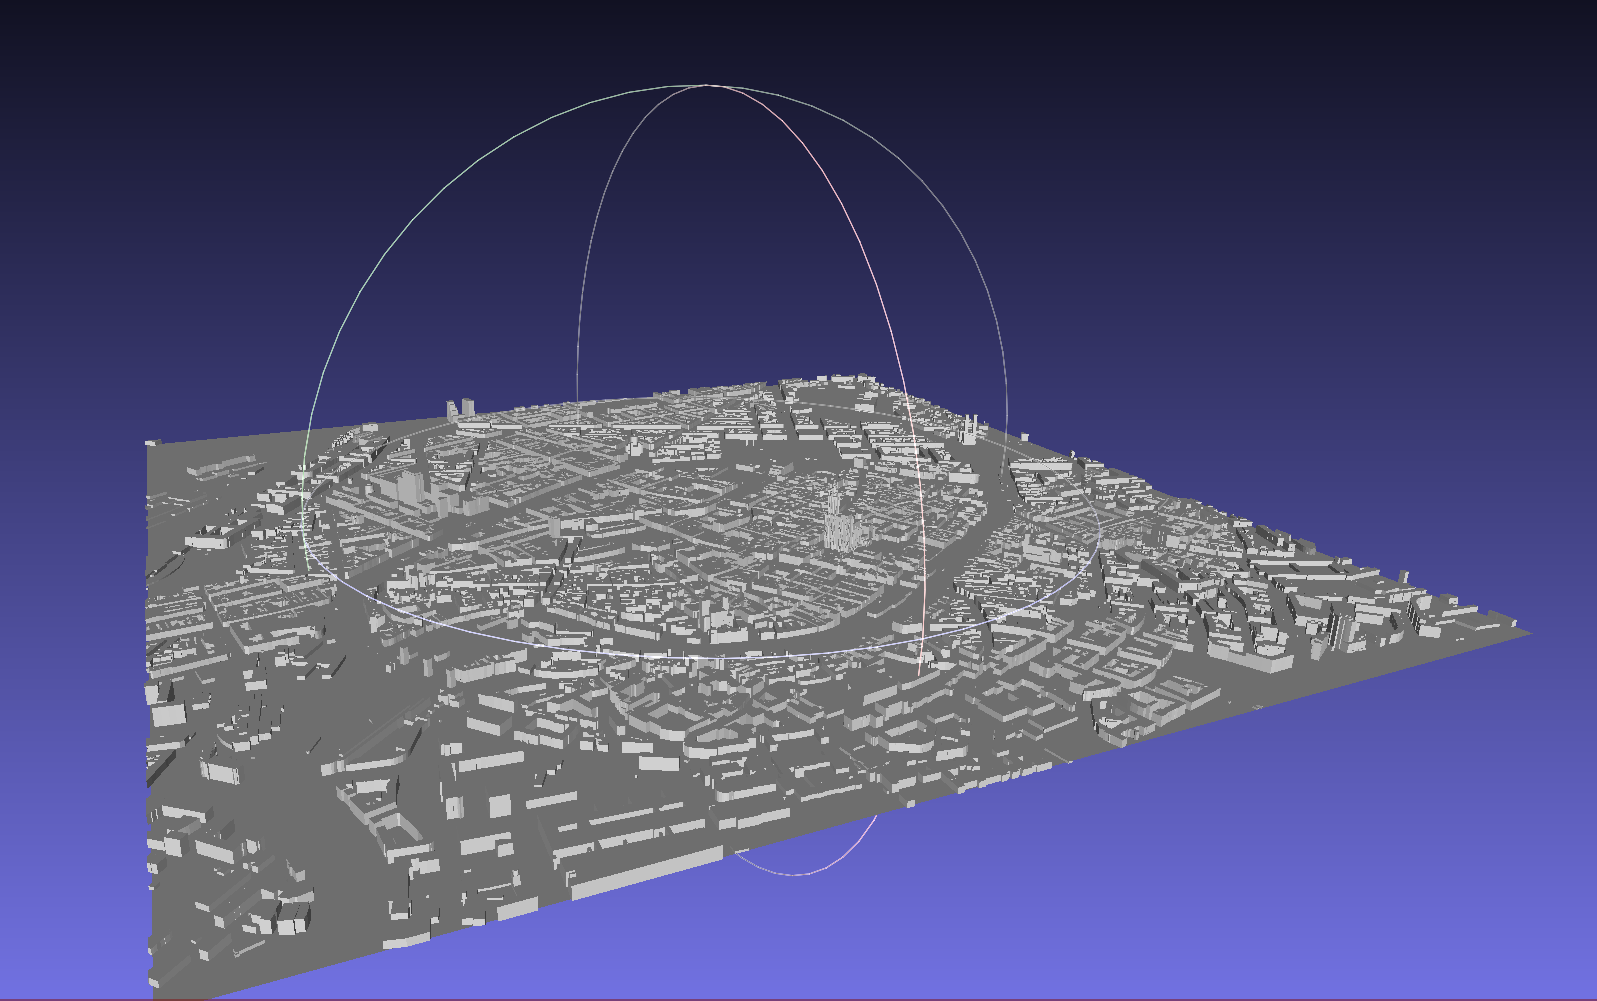
\includegraphics[width=1\textwidth]{images/strasbourg3d.png}
    \captionsetup{font={scriptsize}}
    \caption{Strasbourg 3D model.}
\end{figure}

The idea is to integrate the tree models into the terrain mesh.

\subsection{Shading calculations}
Using \texttt{Feel++} ray tracing, shading effects on buildings will be simulated to account for the presence
of trees and their impact on urban microclimates. Execution time considerations will be
addressed to optimize computational efficiency.

\subsection{Metrics}
The complexity of the algorithms is a key metric to consider. \\
On each execution of the program, basics metrics will be exported to a text file in 
the \texttt{output} directory. \\
These results will be analyzed more thoroughly in the \textbf{Results} section.

Example of the result's metrics for \texttt{grande\_ile\_LOD1.txt}:

\begin{lstlisting}
Area: 561545 meters
Total number of trees: 409
Number of tree which had no height: 67
Number of tree which had no genus: 27
Number of vertices: 241791
Number of faces: 482686
Time to mesh: 155.965 seconds, (2.59942 minutes)
\end{lstlisting}

\section{Implementation}

\subsection{Querying data}
%  data acquisition
%  tree library
%  tree model generation
\begin{lstlisting}[language=C++]
void perform_query(std::string bbox);
nlohmann::json get_query_result();
\end{lstlisting}

We will mainly be using the \texttt{nlohmann json} library (available as a package or as 
header only).

\subsection{Class tree}
\begin{lstlisting}[language=C++]
using K = CGAL::Exact_predicates_inexact_constructions_kernel;
using Point_3 = K::Point_3;
using Mesh = CGAL::Surface_mesh<Point_3>;

class Tree {
    private:
    long M_id;
    double M_lat;
    double M_lon;
    std::string M_genus;
    std::string M_species;
    std::string M_season;
    double M_height;
    double M_circumference;
    double M_diameter_crown;
    double M_x, M_y;
    Mesh M_wrap;
    std::vector<std::string> M_known_genus, M_cedrus_like, M_acer_like,
        M_liquidambar_like, M_quercus_like;

    public:
    void computeXY(double ref_lat, double ref_lon);
    void wrap(int lod);
    void load_data(const std::string &filename);
};

Tree createTreeFromJson(const nlohmann::json &treeJson);
std::ostream &operator<<(std::ostream &os, const Tree &tree);
bool operator<(const Tree &lhs, const Tree &rhs);
\end{lstlisting}

Each tree model has a CGAL \href{https://doc.cgal.org/latest/Surface_mesh/classCGAL_1_1Surface__mesh.html}{Mesh}
wrapper object that will contain the tree's
mesh and its position in the 3D space.

Scaling and moving the trees into the correct position ended being more complex
than expected. \\


\begin{lstlisting}[language=C++]
// Calculate centroid of the tree
double centroid_x = 0, centroid_y = 0, centroid_z = 0;
for (const Point_3 &p : points) {
    centroid_x += p.x();
    centroid_y += p.y();
    centroid_z += p.z();
}
centroid_x /= points.size();
centroid_y /= points.size();
centroid_z /= points.size();
Point_3 centroid(centroid_x, centroid_y, centroid_z);

// Calculate bounding box from points
for (const Point_3 &p : points)
    bbox += p.bbox();

scaling_factor_double = M_height / (bbox.zmax() - bbox.zmin());

K::RT scaling_factor(scaling_factor_double); // Convert to exact type

// Find the base of the tree (minimum z-coordinate)
double base_z = std::numeric_limits<double>::max();
for (const auto &p : points) {
    if (p.z() < base_z)
        base_z = p.z();
}

// Create affine transformations
CGAL::Aff_transformation_3<K> translate_to_base(
    CGAL::TRANSLATION, Vector_3(-centroid.x(), -centroid.y(), -base_z));
CGAL::Aff_transformation_3<K> scale(CGAL::SCALING, scaling_factor);
CGAL::Aff_transformation_3<K> translate_back(
    CGAL::TRANSLATION, Vector_3(centroid.x(), centroid.y(), base_z));
CGAL::Aff_transformation_3<K> translate_to_target(CGAL::TRANSLATION,
                                                  Vector_3(M_x, M_y, 0));

// Apply transformations: move to base, scale, move back, move to target
for (auto &p : points) {
    p = translate_to_base.transform(p);   // Move to base
    p = scale.transform(p);               // Scale
    p = translate_back.transform(p);      // Move back to original position
    p = translate_to_target.transform(p); // Move to target position
}
// Clear existing mesh data
M_wrap.clear();

// Add transformed vertices to the mesh and store their descriptors
std::map<Point_3, Mesh::Vertex_index> vertex_map;
for (const auto &p : points) {
    auto v = M_wrap.add_vertex(p);
    // Store the vertex descriptor for the transformed vertex
    vertex_map[p] = v;
}

// Add faces to the mesh
for (const auto &face : faces) {
    // Retrieve vertex descriptors for the face vertices
    Mesh::Vertex_index v0 = vertex_map[points[face[0]]];
    Mesh::Vertex_index v1 = vertex_map[points[face[1]]];
    Mesh::Vertex_index v2 = vertex_map[points[face[2]]];

    // Add the face to the mesh
    M_wrap.add_face(v0, v1, v2);
}
\end{lstlisting}

To ensure the placement was correct we first had to move the tree to the origin
of its bounding box, scale it to the correct height, move it back to its original position
(because scaling it was moving the tree around), and finally move it to the correct position in the 3D space.
%  model integration
%  shading calculations

\section{Results}


\newpage

\section{Conclusion}


\newpage

\section{References}
\bibliographystyle{unsrt}
\bibliography{references}

\end{document}
